\documentclass[crop,tikz]{standalone}
\usetikzlibrary{backgrounds}
\colorlet{blue}{cyan}
\tikzset{
  inverted/.style = {
    color=white,
    background rectangle/.style={fill},
    show background rectangle
  }
}

\usepackage{pgfplots}
\tikzset{>=latex}

\pgfplotsset{
  compat=1.16,
  every non boxed x axis/.append style={
    axis line style={-latex}
  },
  every non boxed y axis/.append style={
    axis line style={-latex}
  },
  inverted/.style = {
    every axis legend/.append style={
      draw=white,
      fill=black,
      text=white
    }
  }
}

\begin{document}
  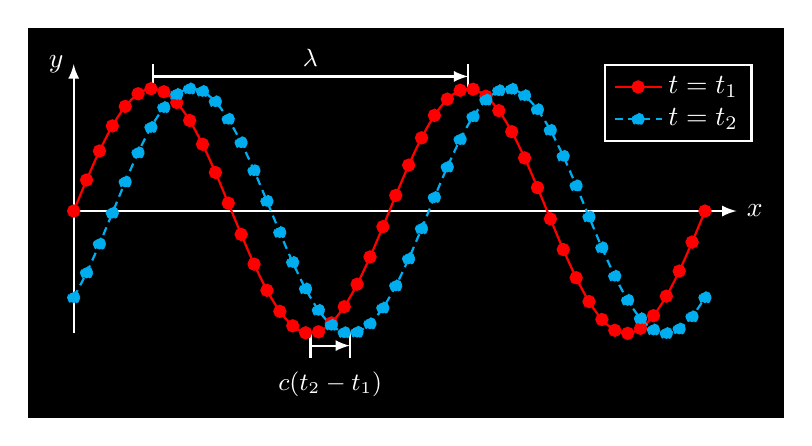
\begin{tikzpicture}[inverted,inverted]
    \begin{axis}[inverted,
      thick,
      width=10cm,
      height=5cm,
      domain=0:{4*pi},
      samples=50,
      axis y line=middle,
      axis x line=middle,
      xmax={4.2*pi},
      ymax=1.2,
      xlabel={$x$},
      ylabel={$y$},
      xlabel style={right},
      ylabel style={left},
      ticks=none,
      legend cell align={left},
      legend style={at={(0.8,1)},anchor=north west},
      clip=false,
      ]
      \addplot[red,mark=*,smooth] {sin(deg(x))};
      \addplot[blue,mark=*,smooth,densely dashed] {sin(deg(x - pi/4))};
      \legend{$t=t_1$, $t=t_2$};
      \draw[thick,->] (axis cs:1.5*pi,-1.1) -- node[below,yshift=-0.2cm] {\small $c(t_2-t_1)$} (axis cs:7*pi/4,-1.1);
      \draw[] (axis cs:1.5*pi,-1) -- (axis cs:1.5*pi,-1.2);
      \draw[] (axis cs:7*pi/4,-1) -- (axis cs:7*pi/4,-1.2);
      \draw[thick,->] (axis cs:pi/2,1.1) -- node[above] {\small $\lambda$} (axis cs:2.5*pi,1.1);
      \draw[] (axis cs:pi/2,1) -- (axis cs:pi/2,1.2);
      \draw[] (axis cs:2.5*pi,1) -- (axis cs:2.5*pi,1.2);
    \end{axis}
  \end{tikzpicture}
\end{document}
